\chapter{Direct Switching Power Supply (Asymmetric FORWARD)}
The purpose of this problem is the simplified study of the switching converter represented in the following figure:

\begin{figure}[h]
\centering
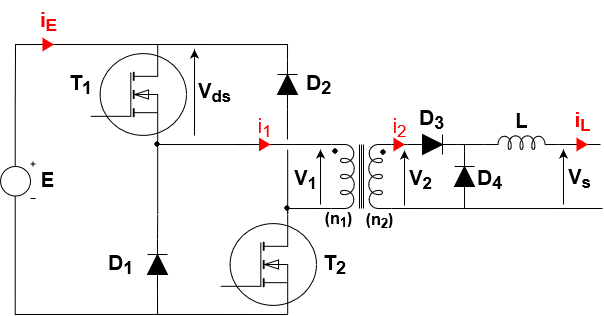
\includegraphics[width=0.85\linewidth]{TD_Forward_Asymetrique/fig/Forward_Asymetrique.png}
\end{figure}

All the semiconductors are assumed to be perfect. The two windings of the transformer are made on the same ferromagnetic core without leakage: all the turns "enclose" the same elementary flux $\varphi$, and the reluctance of this magnetic circuit is denoted by $R$. The output inductance coil $L$ is independent of this transformer. All resistances are neglected.

The control of the transistors is identical, performed at the period $T$, with a duty cycle denoted by $\alpha$: they are therefore conductive
during the interval $[0,\ \alpha.T]$, and blocked during the interval $[\alpha.T,\ T]$.

The output voltage $V_s$ is assumed to be constant throughout the study, and the device will be kept in total demagnetization at each operating cycle. We are only interested in the continuous conduction mode in the output inductance $L$, so its current never becomes zero: $i_L > 0$.

\begin{enumerate}
\item \textbf{General operation of the power supply}

In this part, we will study the operation of the power supply. We will assume that it operates in \textbf{total demagnetization}, meaning that at the end of a period, the magnetic flux in the transformer is zero. We will plot the time curves of $\varphi$ (magnetic flux in the transformer), $v_1$, $v_2$, $v_{DS}$ (drain-source voltage of transistor $T_1$), $v_L$, $i_1$, $i_2$, $i_L$, and $i_E$.

\begin{enumerate}

\item Considering the directions of the windings shown in the diagram and the directions of measurement of the different currents and voltages:
\begin{enumerate}
\item Give the expression of the voltages $v_1$ and $v_2$ as a function of the flux $\varphi$
\item Express the Hopkinson's law relating the currents $i_1$ and $i_2$ to the same flux $\varphi$ using the number of turns and the reluctance $R$.
\end{enumerate}

\item We consider the interval $[0,\ \alpha T]$: we assume that the initial flux at $t = 0$ is zero (total demagnetization)
\begin{enumerate}
\item Determine the voltage $v_1$ applied to the primary winding
\item Deduce the voltage $v_2$ as well as the state of diodes $D3$ and $D4$
\item Give the expression of the voltage $v_L$ across the output inductance in terms of the number of turns, $E$, and $V_S$
\item Express the evolution of the flux $\varphi (t)$ during this time interval
\item Express the current $i_2$ in terms of $i_L$
\item Using the Hopkinson's law and the previous results, determine the expression of the primary current $i_1$ in terms of $i_L$ and the flux $\varphi$ using the number of turns and the reluctance $R$
\item At the instant $\alpha T$, the end of this first time interval, we assume that the flux has become equal to $\varphi_0$. Deduce the expression of this value of $\varphi_0$ in terms of $E$, $n_1$, and $\alpha T$
\end{enumerate}

\item We consider the interval $[\alpha T,\ T]$: all transistors are blocked.
\begin{enumerate}
\item At $t=\alpha T$, determine the state of diodes $D1$ and $D2$. What are the values of voltages $v_1$ and $v_2$? Deduce the state of diodes $D3$ and $D4$
\item Deduce the expression of $v_L$ in terms of $V_S$
\item Express the evolution of the flux $\varphi(t)$ during this time interval
\item At what instant $t_0$ does the flux become zero? Give a condition on $\alpha$ for the system to operate in total demagnetization
\item What happens next until the end of the period T?
\end{enumerate}

\item The power supply is intended to produce a constant voltage of 24 V from the perfectly filtered single-phase rectified network, $E = 300 V$. The transmitted power is $P_n = 600 W$, and the switching frequency is $f = 50 kHz$. We choose to operate the power supply around the nominal duty cycle $\alpha = 0.4$.
\begin{enumerate}
\item Calculate the turns ratio $n_2/n_1$
\item Calculate the average value $I_s$ of the current $i_L$
\item Calculate the minimum value to be given to the inductance $L$ to limit the peak-to-peak ripple of the current $i_L$ to 5\% of its average value $I_s$. \underline{Keep this} \underline{value of $L$ for the following calculations}
\item Deduce the maximum value $I_{1\ max}$ of the current in the transistor when neglecting the magnetizing current
\end{enumerate}

\end{enumerate}

\item \textbf{Transformer dimensioning}

\begin{enumerate}
\item To justify the previous assumption, determine the minimum value of the magnetizing inductance $L_1$ (seen from the primary winding) that makes the maximum no-load current less than $I_{1\ max} /20$

\item \underline{Neglecting the ripple of the current $i_L$ and the magnetizing current}, determine the rms values $I_{1\ eff}$ and
$I_{2\ eff}$ of the currents $i_1$ and $i_2$ in terms of $I_s$, $n_1$, $n_2$, and $\alpha$
\item Determine, with these same assumptions, the minimum winding area $S_B$ required in terms of current density $\delta$, winding coefficient $k_B$, $I_s$, $n_2$, and $\alpha$
\item Also give the expression of the minimum cross-sectional area $A_e$ of the core that avoids core saturation by maintaining a maximum induction below $B_{max}$
\item Deduce the minimal sizing product $A_e.S_B$ of this transformer in terms of the duty cycle, the different characteristic parameters of this power supply, including its output power $P_S$, and its switching frequency $f$

\end{enumerate}

\end{enumerate}

\begin{figure}[h]
\centering
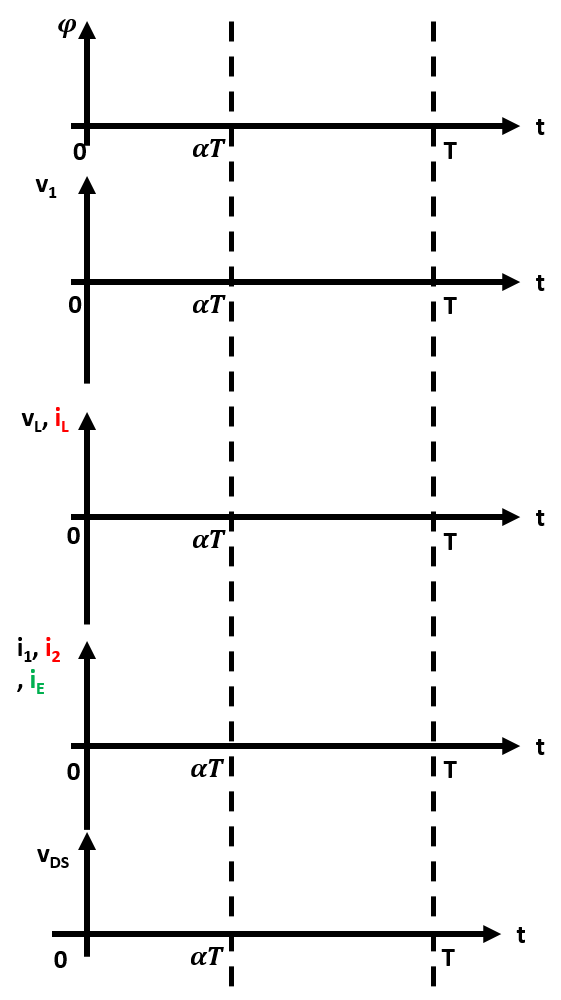
\includegraphics[width=0.85\linewidth]{TD_Forward_Asymetrique/fig/doc_reponse.png}
\end{figure}
